\chapter{Testing and Experimental Results}
\label{cap:cap4}

This chapter presents the testing methodology and results. The platform was tested at two levels: automated unit tests for individual components and manual end-to-end tests to verify the complete workflow.

The purpose of testing is to verify that each component works correctly on its own (unit tests) and that all components work together as a complete system (manual tests). Unit tests are fast, repeatable and can be run automatically. Manual tests are slower but they test real scenarios with actual Docker containers, network communication and user interaction.

The test environment consists of a single macOS machine (Apple Silicon, 11 CPU cores, 18 GB RAM) running Docker Desktop. The master and workers run as separate processes on the same machine, communicating through localhost.

\section{Unit Tests}

Unit tests verify that individual components work correctly in isolation. Each test creates the needed objects in memory, calls a function and checks that the result is correct. The tests are written in Go using the standard \texttt{testing} package and can be run with \texttt{go test ./...}. No external services (Docker, network) are needed for unit tests.

\subsection{Load Balancer Tests}

Four tests verify the LeastConnections and Weighted strategies:

\begin{itemize}
    \item \textbf{TestLeastConnections\_SelectsNodeWithFewestContainers}. Given 3 nodes with 5, 2 and 8 containers respectively, the load balancer selects the node with 2 containers.
    \item \textbf{TestLeastConnections\_EmptyCandidates}. When no candidates are provided, returns nil.
    \item \textbf{TestWeighted\_SelectsNodeWithMostResources}. Given 3 nodes with different CPU/RAM usage, the load balancer selects the node with the highest available resources (87\% CPU free, 87\% RAM free).
    \item \textbf{TestWeighted\_EmptyCandidates}. When no candidates are provided, returns nil.
\end{itemize}

\subsection{Scheduler Tests}

Three tests verify the scheduling logic:

\begin{itemize}
    \item \textbf{TestSchedule\_FindsNode}. With one alive node that has enough resources, the scheduler returns it.
    \item \textbf{TestSchedule\_NotEnoughResources}. When the service requires 100 CPU cores but the node only has 6 available, the scheduler returns an error.
    \item \textbf{TestSchedule\_EmptyPool}. When the pool has no nodes, the scheduler returns an error.
\end{itemize}

\subsection{ACL Tests}

Four tests verify the role-based access control:

\begin{itemize}
    \item \textbf{TestAdminCanDoEverything}. Admin can create, delete and read services, nodes, users and audit.
    \item \textbf{TestReaderCannotCreate}. Reader cannot create or delete services.
    \item \textbf{TestWriterCannotManageUsers}. Writer cannot create users.
    \item \textbf{TestInvalidRole}. An unknown role has no permissions.
\end{itemize}

\subsection{Results}

All unit tests pass:

\begin{verbatim}
$ go test ./internal/loadbalancer/ ./internal/scheduler/ ./internal/security/ -v

--- PASS: TestLeastConnections_SelectsNodeWithFewestContainers
--- PASS: TestLeastConnections_EmptyCandidates
--- PASS: TestWeighted_SelectsNodeWithMostResources
--- PASS: TestWeighted_EmptyCandidates
ok   internal/loadbalancer

--- PASS: TestSchedule_FindsNode
--- PASS: TestSchedule_NotEnoughResources
--- PASS: TestSchedule_EmptyPool
ok   internal/scheduler

--- PASS: TestAdminCanDoEverything
--- PASS: TestReaderCannotCreate
--- PASS: TestWriterCannotManageUsers
--- PASS: TestInvalidRole
ok   internal/security
\end{verbatim}

\section{Manual Testing}

The following scenarios were tested manually to verify the end-to-end behavior of the platform. Each test follows the same structure: an objective describing what is being verified, the steps to reproduce the test, the expected result with specific details about what the output should look like and a screenshot showing the actual result.

\subsection{Node Discovery and Heartbeats}

\textbf{Objective:} Verify that worker nodes are discovered automatically when they start sending heartbeats and that the master correctly displays their status and metrics.

\textbf{Steps:}
\begin{enumerate}
    \item Start the master: \texttt{./bin/master -raft-bootstrap}
    \item Start worker-1: \texttt{./bin/worker -id worker-1 -addr localhost:7001}
    \item Start worker-2: \texttt{./bin/worker -id worker-2 -addr localhost:7002}
    \item Wait 10 seconds and observe the master log.
\end{enumerate}

\textbf{Expected result:} The master log shows ``new node discovered'' for each worker within 5 seconds of starting. The cluster status display (every 10 seconds) lists both workers with status ALIVE, their CPU and RAM usage and the time since their last heartbeat. This confirms that auto-join works and that heartbeats are being received correctly.

\begin{figure}[H]
    \centering
    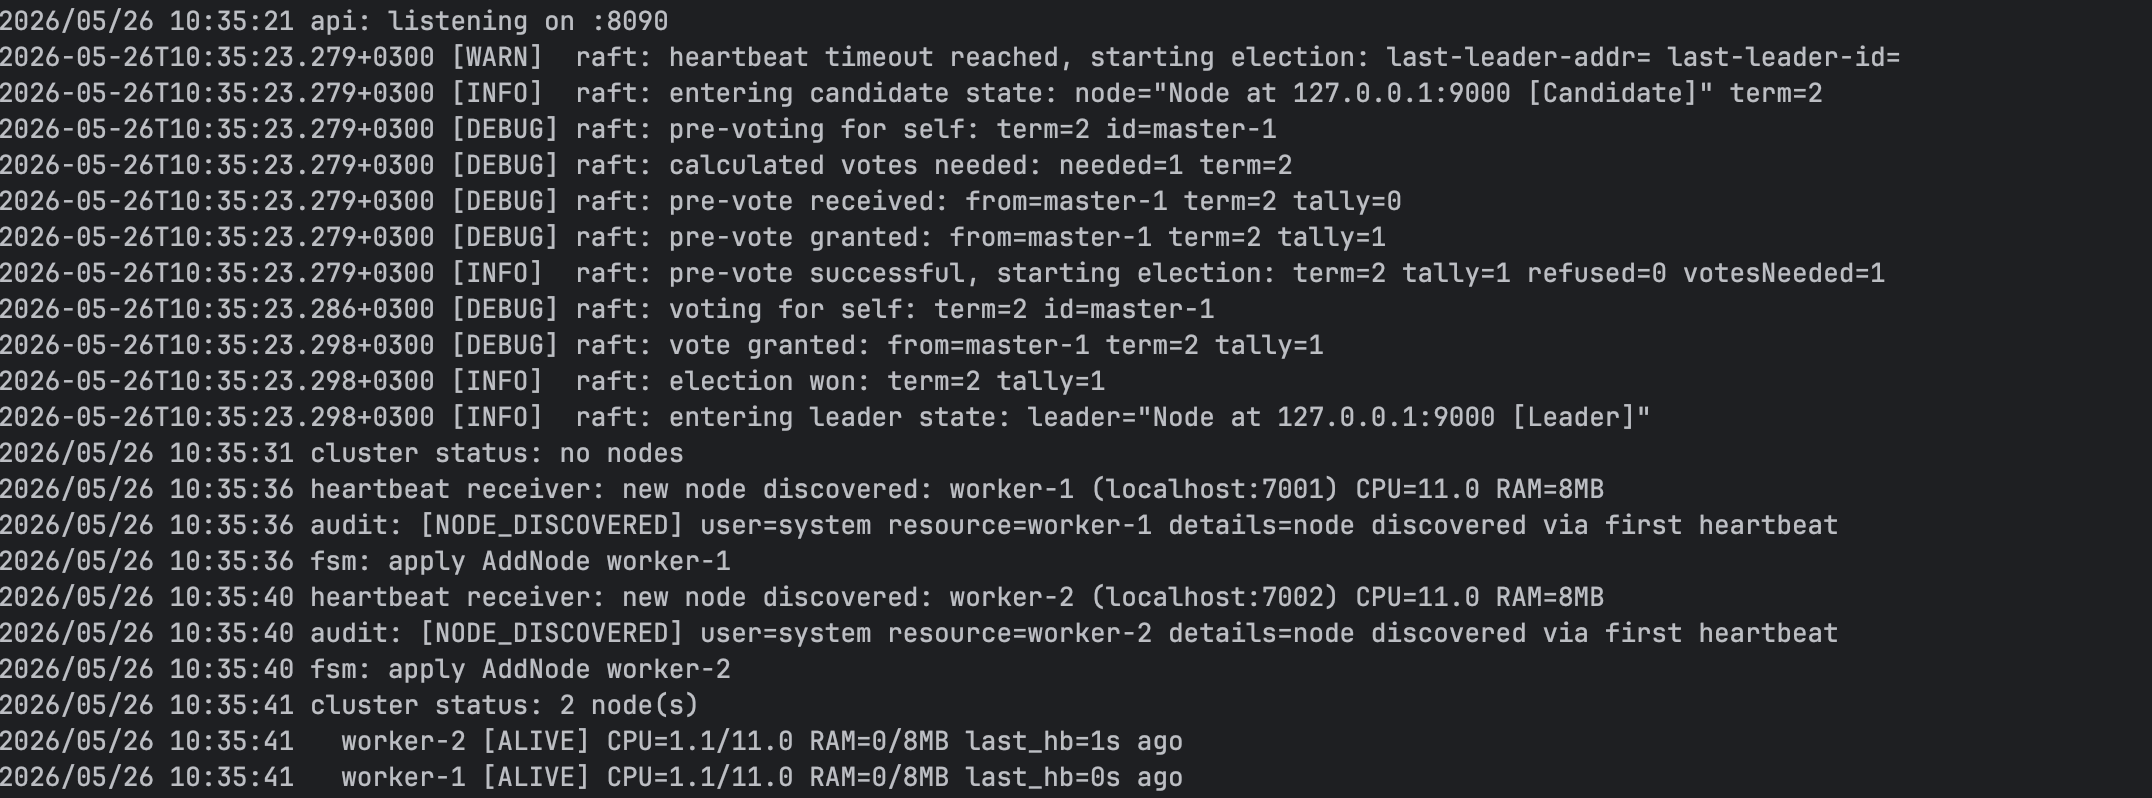
\includegraphics[width=\textwidth]{continut/capitol4/figuri/test_discovery.png}
    \caption{Node discovery: two workers auto-joined the cluster}
    \label{fig:test_discovery}
\end{figure}

\subsection{Service Deployment}

\textbf{Objective:} Verify that a user can authenticate, deploy a service and that the container is actually running on Docker.

\textbf{Steps:}
\begin{enumerate}
    \item Login as admin: \texttt{curl -X POST http://localhost:8090/login -d '\{"username":"admin","password":"admin"\}'}
    \item Deploy nginx using the access token from step 1: \texttt{curl -X POST http://localhost:8090/services -H "Authorization: Bearer <TOKEN>" -d '\{"name":"nginx","image":"nginx:latest","cpu":0.5,"ram":256,"replicas":1,"pool":"high-cpu"\}'}
    \item Verify the container is running: \texttt{docker ps}
\end{enumerate}

\textbf{Expected result:} The login returns a JSON with \texttt{accessToken}, \texttt{refreshToken} and \texttt{expiresIn} (900 seconds). The deploy returns 201 Created with a \texttt{serviceID} and a \texttt{containers} array where each container has status RUNNING and a \texttt{nodeID}. The \texttt{docker ps} command shows a container named \texttt{dcp-<serviceID>} running on the machine.

\begin{figure}[H]
    \centering
    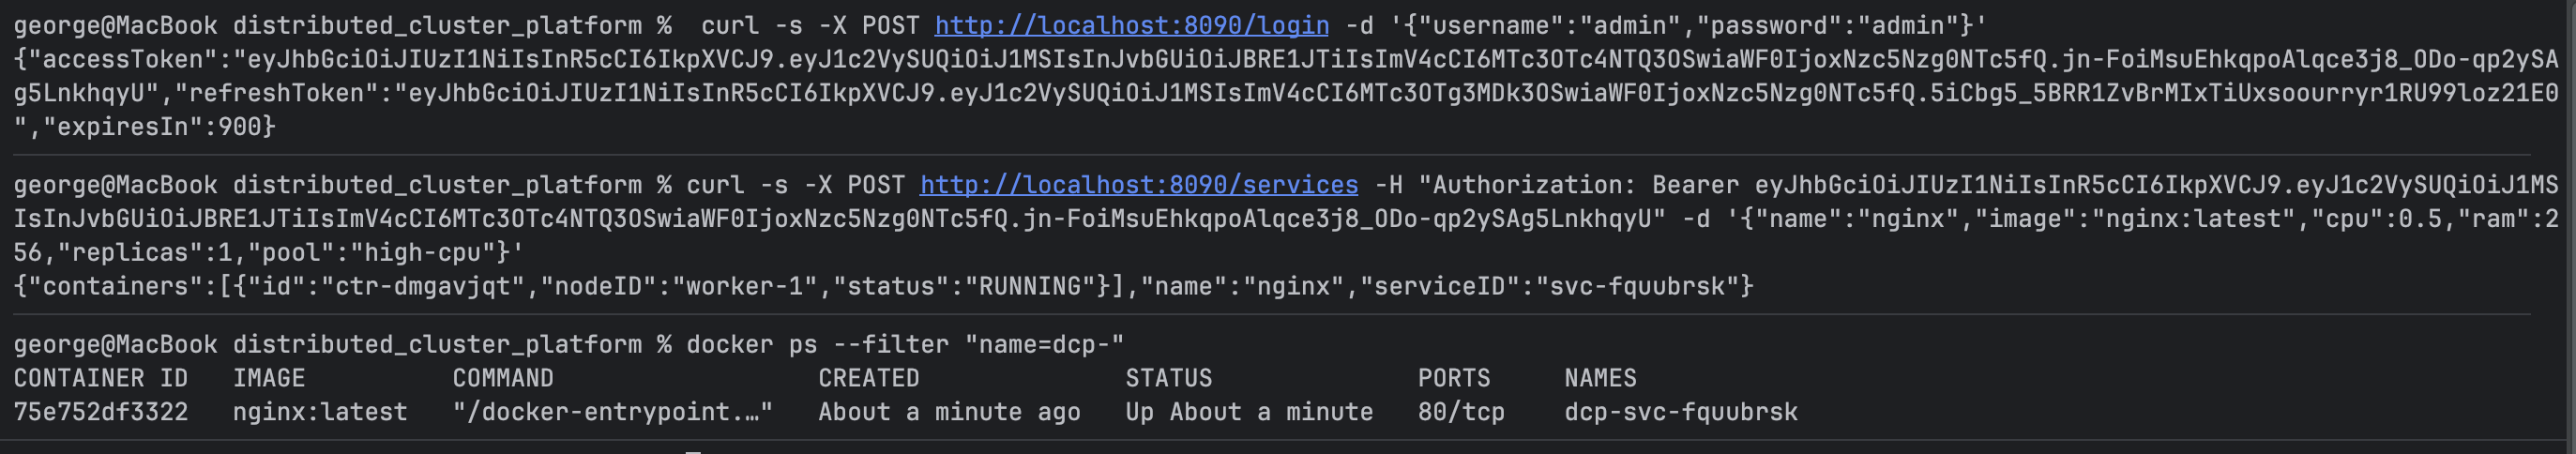
\includegraphics[width=\textwidth]{continut/capitol4/figuri/test_deploy.png}
    \caption{Service deployment: nginx container running on worker-1}
    \label{fig:test_deploy}
\end{figure}

\subsection{Fault Tolerance}

\textbf{Objective:} Verify that the master detects a failed node, transitions it through SUSPECT and DEAD states and handles split-brain when the node recovers.

\textbf{Steps:}
\begin{enumerate}
    \item With both workers running, stop worker-1 with Ctrl+C.
    \item Wait 15 seconds and observe SUSPECT in the master log.
    \item Wait 30 seconds and observe DEAD in the master log.
    \item Restart worker-1: \texttt{./bin/worker -id worker-1 -addr localhost:7001}
    \item Observe KillContainers in the master and worker logs.
\end{enumerate}

\textbf{Expected result:} After 15 seconds without heartbeat, the master log shows ``node worker-1 marked SUSPECT''. After 30 seconds, it shows ``node worker-1 marked DEAD''. When worker-1 is restarted, the master log shows ``late heartbeat from DEAD node worker-1, sending KillContainers'' followed by ``node worker-1 back to ALIVE''. The worker log confirms it received the KillContainers command. This verifies the complete fault tolerance cycle.

\begin{figure}[H]
    \centering
    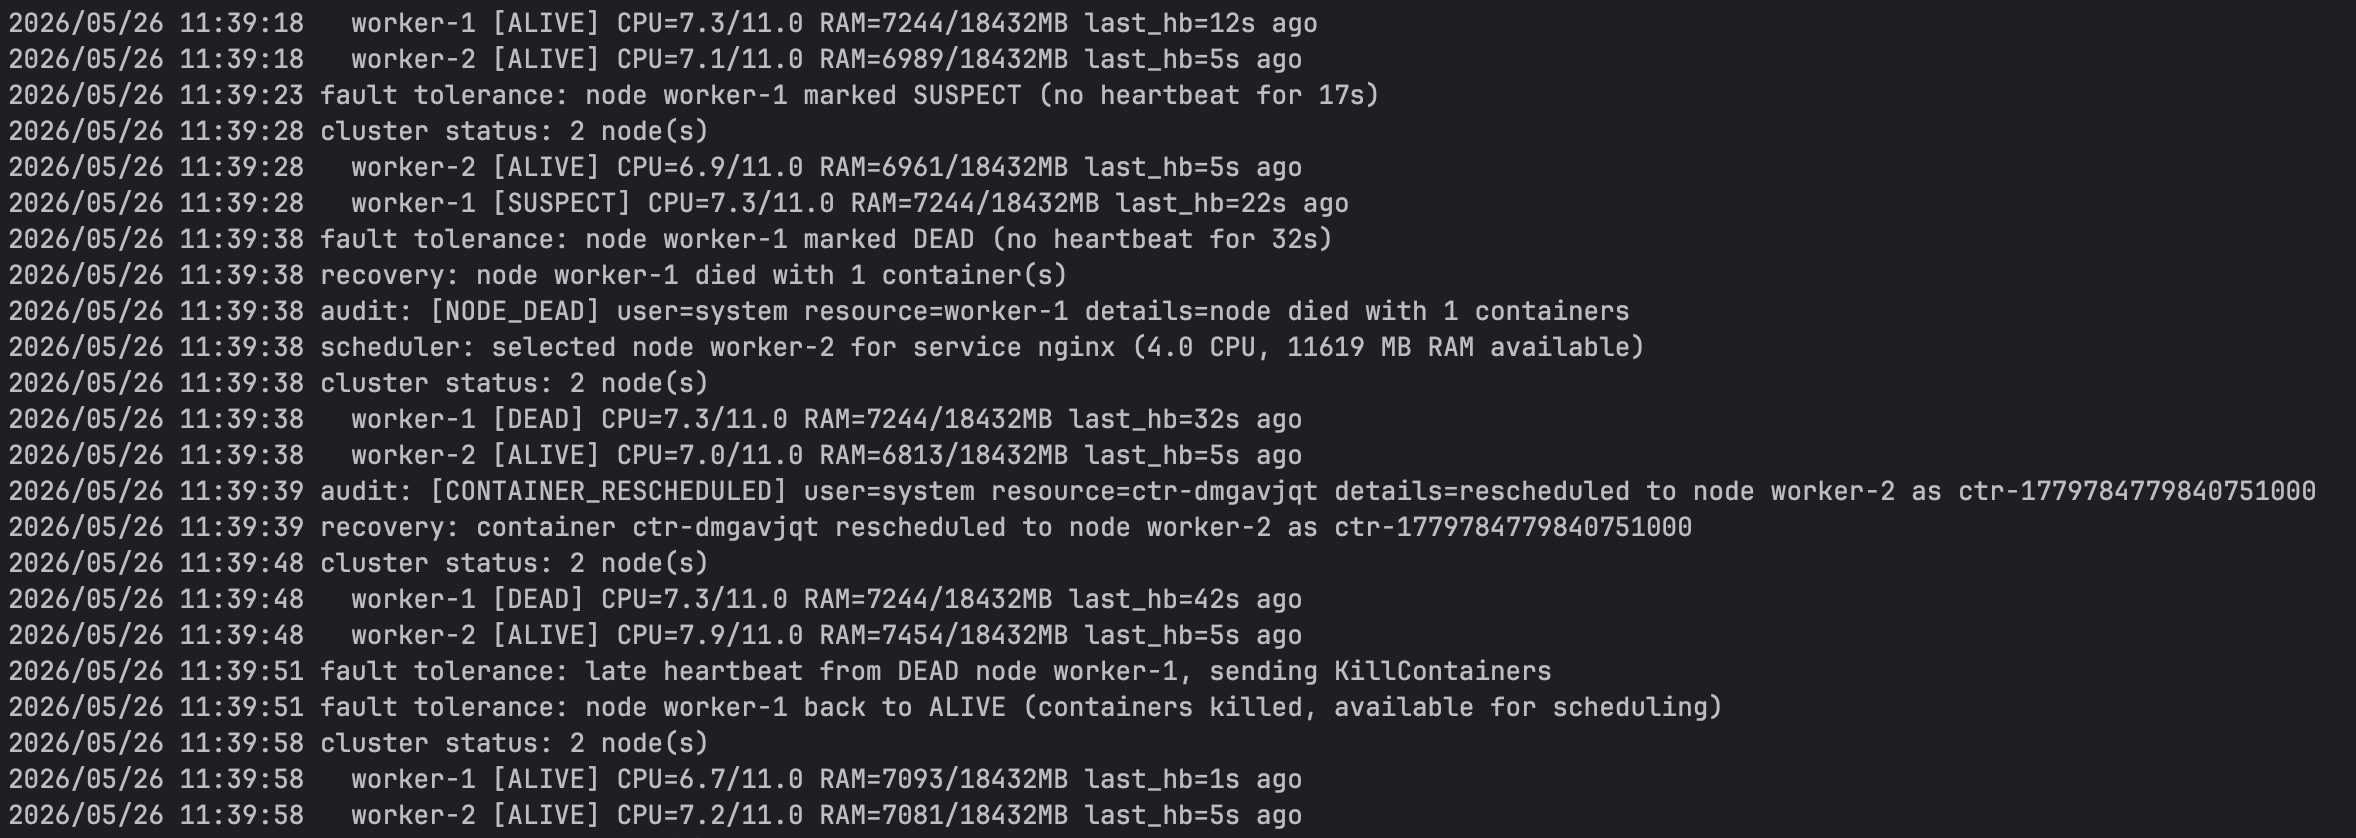
\includegraphics[width=\textwidth]{continut/capitol4/figuri/test_fault.png}
    \caption{Fault tolerance: node marked SUSPECT, then DEAD, then recovered}
    \label{fig:test_fault}
\end{figure}

\subsection{Security: Role-Based Access Control}

\textbf{Objective:} Verify that the READER role cannot create services while the ADMIN role can.

\textbf{Steps:}
\begin{enumerate}
    \item Login as reader: \texttt{curl -X POST http://localhost:8090/login -d '\{"username":"reader","password":"reader"\}'}
    \item Try to deploy a service using the reader token.
    \item Login as admin and deploy the same service.
\end{enumerate}

\textbf{Expected result:} The reader login succeeds but the deploy request returns 403 Forbidden with the error ``role READER cannot create services''. The master log shows an AUTH\_DENIED audit event. The admin login and deploy succeed with 201 Created. This confirms that the ACL middleware correctly enforces role-based permissions.

\begin{figure}[H]
    \centering
    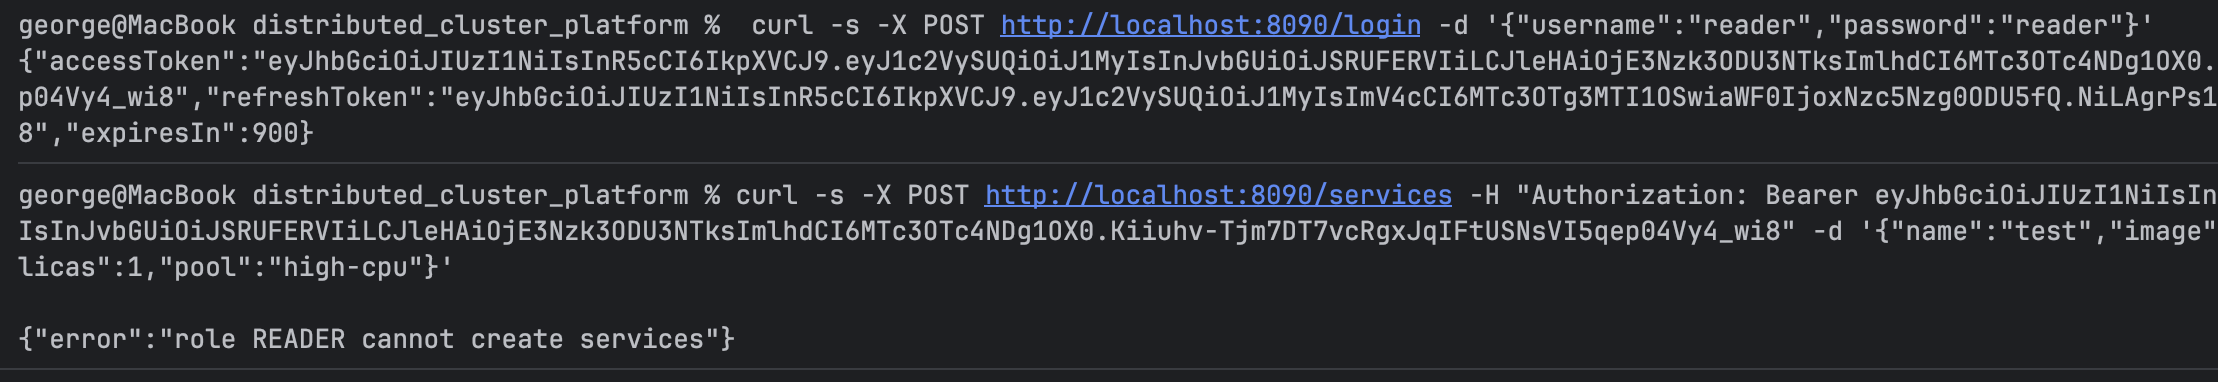
\includegraphics[width=\textwidth]{continut/capitol4/figuri/test_security.png}
    \caption{Security: reader denied, admin allowed}
    \label{fig:test_security}
\end{figure}

\subsection{Audit Log}

\textbf{Objective:} Verify that all important actions are recorded in the audit log and that the log can be queried with filters.

\textbf{Steps:}
\begin{enumerate}
    \item Perform several actions: login, deploy a service, delete a service.
    \item Query the full audit log: \texttt{curl -H "Authorization: Bearer <TOKEN>" http://localhost:8090/audit}
    \item Query with a filter: \texttt{curl -H "Authorization: Bearer <TOKEN>" http://localhost:8090/audit?action=LOGIN}
\end{enumerate}

\textbf{Expected result:} The audit log returns a JSON array of events. Each event has a timestamp, user ID, action type (LOGIN, SERVICE\_CREATE, NODE\_DISCOVERED, AUTH\_DENIED, etc.) and the affected resource. The filtered query returns only events matching the specified action. The log is append-only, so all events from the current session are present in chronological order.

\begin{figure}[H]
    \centering
    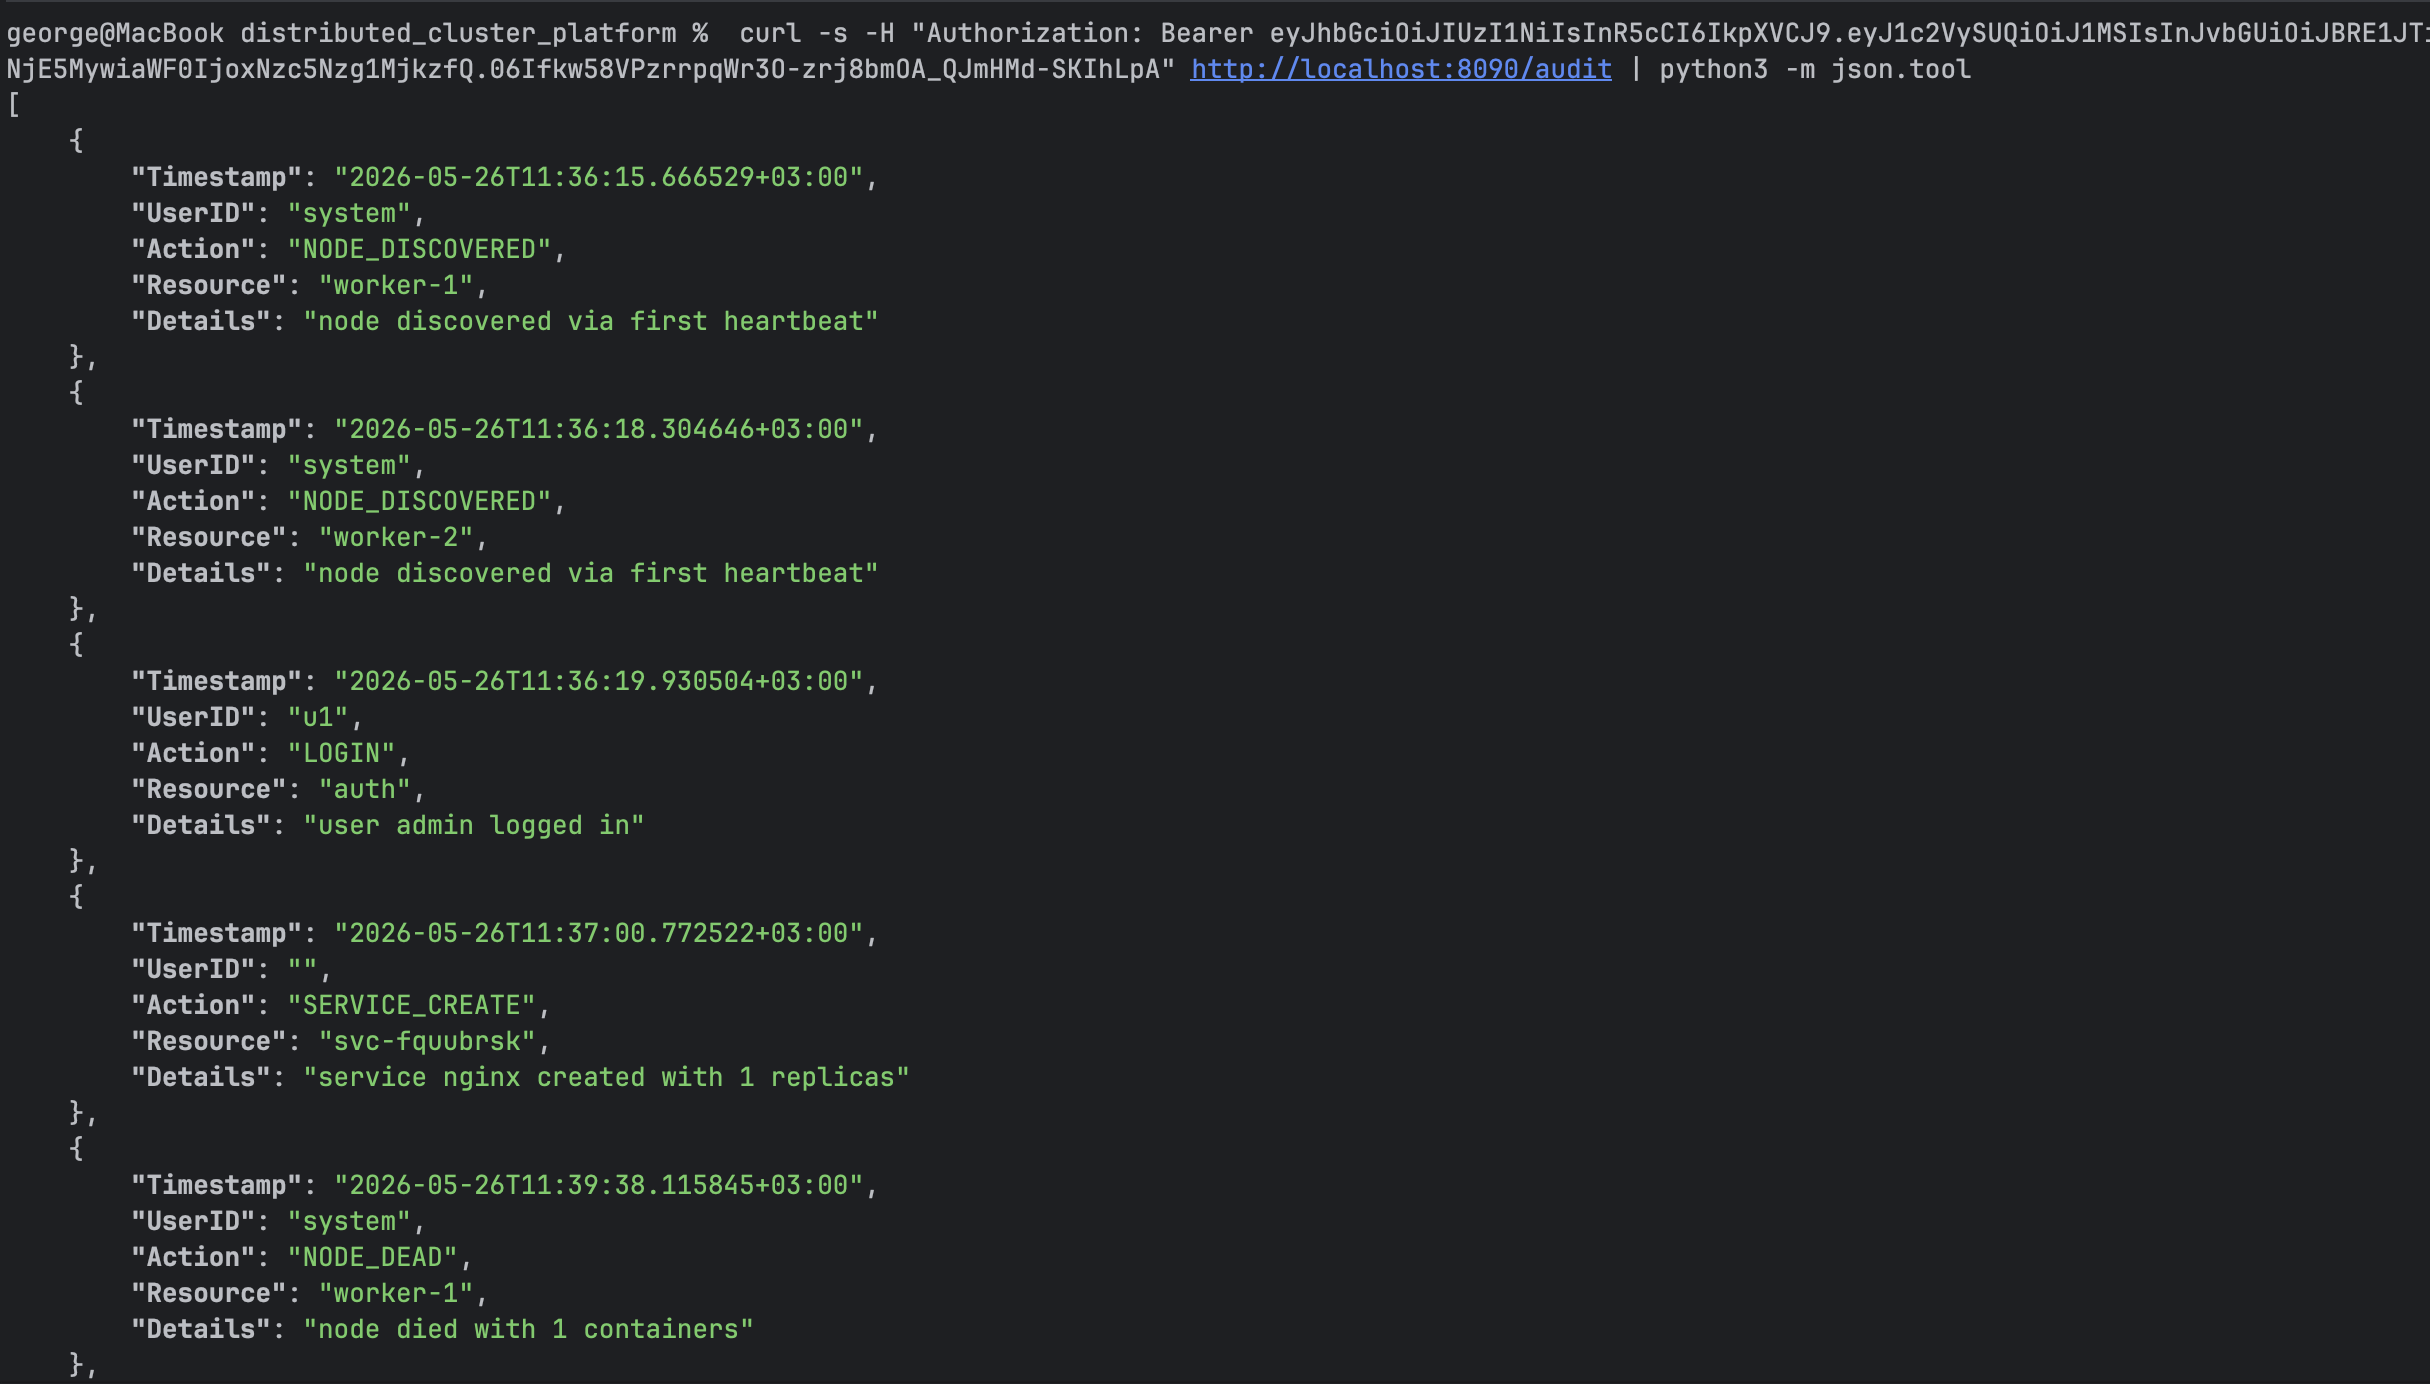
\includegraphics[width=\textwidth]{continut/capitol4/figuri/test_audit.png}
    \caption{Audit log with recorded events}
    \label{fig:test_audit}
\end{figure}